\documentclass[aspectratio=169,11pt]{beamer}
\usepackage{beamertemplate}
\usepackage{graphicx}
\usepackage{url}
\usepackage{textcomp}
\usepackage{eurosym}
\usepackage[normalem]{ulem}
\usepackage{ragged2e}
\usepackage{etoolbox}
\apptocmd{\itemize}{\justifying}{}{}
\AtBeginEnvironment{frame}{\justifying}

% Repite el índice al empezar cada sección, resaltando la que comienza
\setbeamertemplate{section in toc shaded}[default][30]
\AtBeginSection[]{%
  \begin{frame}{Índice}
  \footnotesize
  \tableofcontents[currentsection]
  \end{frame}
}

\title[SSI -- Tema 2.2]{Escaneo, Fingerprinting y Técnicas de Evasión}
\subtitle{Seguridad en Sistemas Informáticos --- Tema 2.2}
\author{José Luis Martínez}
\institute{Universidad de Castilla-La Mancha}
\date{Curso 2026/27}

\begin{document}

\begin{frame}[plain]\titlepage\end{frame}

\section{Introducción}

\begin{frame}{Introducción}
\begin{center}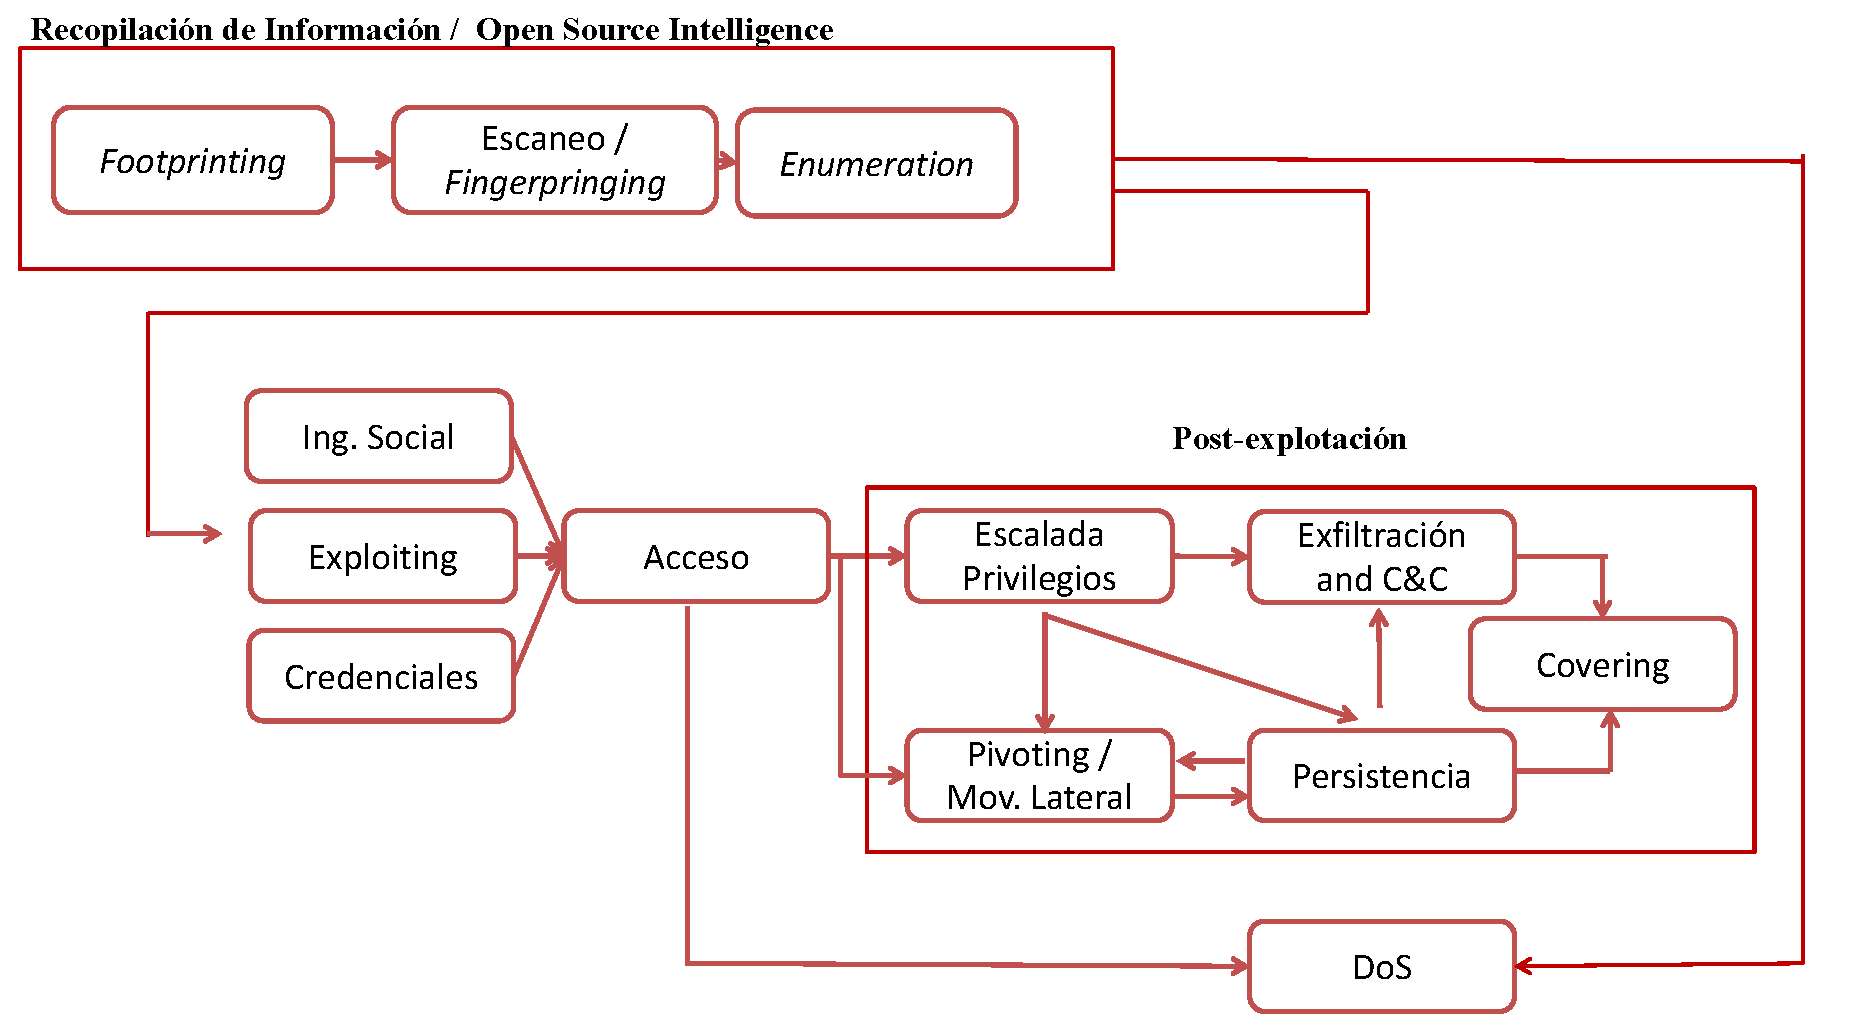
\includegraphics[width=\textwidth,height=0.82\textheight,keepaspectratio]{img/taxonomia-ataque.pdf}
\end{center}
\end{frame}


\begin{frame}[allowframebreaks]{Introducción}
\small
  \begin{itemize}
  \item Tras la fase de footprinting y OSINT, encontraremos mucha información útil para determinar cuál es el mejor vector de ataque. Entre esa información, están los activos relacionados con IPs, rangos de red, sistemas autónomos, dominios, subdominios, DNS, servidores. En este punto es cuando interviene la fase de escaneo, fingerprinting y las técnicas de evasión.
  \item Escaneo consiste en determinar qué hosts / IPs / endpoints están activos y son accesibles (escaneo de hosts) y, para cada uno de los hosts activos, determinar qué puertos están abiertos (escaneo de puertos).
  \item Fingerprinting se refiere a determinar la huella o firma que hay detrás de esos puertos o sistemas, es decir, determinar el sistema operativo (fingerprinting OS) y determinar qué versión (software) hay corriendo detrás de los puertos abiertos.
  \item Las técnicas de evasión consisten en intentar evadir los sistemas de detección y protección que pueda tener el objetivo, como firewalls, IPS/IDS, WAF, etcétera.
  \end{itemize}
\end{frame}

\begin{frame}[allowframebreaks]{Introducción}
\small
  \begin{itemize}
  \item Estas técnicas se engloban en la fase de `recopilación de información' dentro del proceso de auditoría/pentesting/red team/hacking ético, y su principal objetivo es obtener información detallada sobre los sistemas y versiones de los servicios que están corriendo.
  \item Se podría decir que esta fase sirve para identificar al detalle los activos que vamos a auditar para, posteriormente, identificar posibles vulnerabilidades, deficiencias o malas configuraciones que puedan permitir algún tipo de acción ofensiva en el activo.
  \item Antes de pasar a la fase de enumeración de los sistemas y servicios, es imprescindible que tengamos bien definidos cuáles son realmente los activos acotados dentro del alcance de las pruebas.
  \end{itemize}
\end{frame}

\begin{frame}[allowframebreaks]{Introducción}
\small
  \begin{itemize}
  \item Se realiza tanto en auditorías internas como externas, aunque dependiendo del tipo se realizarán unas u otras pruebas de las expuestas a continuación.
  \item Nuestro objetivo durante la realización de esta fase será obtener:
    \begin{itemize}
    \item Información de red:
      \begin{itemize}
      \item {[}Previa] Tener identificados los rangos de red y AS (Sistemas Autónomos).
      \item Identificar información detallada sobre los sistemas activos (SO, servicios, \dots{}).
      \end{itemize}
    \item Información de aplicaciones y dominios:
      \begin{itemize}
      \item {[}Previa] Tener identificados los dominios y subdominios (+ apps).
      \item Identificar información detallada sobre las aplicaciones y servicios activos en dichos dominios.
      \end{itemize}
    \end{itemize}
  \end{itemize}
\end{frame}

\begin{frame}[allowframebreaks]{Introducción}
\small
  \begin{itemize}
  \item Al igual que ocurre con los tipos de ataques, tenemos también dos tipos diferentes de enumeración según la interacción que tengamos con el objetivo:
    \begin{itemize}
    \item Pasivo: se obtiene información sin interacción con el objetivo. Útil en labores de auditoría externa principalmente. La mayoría de las técnicas se vieron en el tema 2.1 anterior.
    \item Activo: se busca obtener información interactuando con el objetivo. Útil en cualquier labor de auditoría externa e interna. Nos permitirá en muchas ocasiones corroborar la información extraída de forma pasiva.
    \end{itemize}
  \end{itemize}
\end{frame}


\section{Escaneo \& Fingerprinting}

\begin{frame}[allowframebreaks]{Escaneo}
\small
  \begin{itemize}
  \item Obtener toda la información que necesitamos de manera pasiva no siempre es posible, además de que muchas veces el alcance pasivo está muy limitado; por ello se vuelve necesario en muchas ocasiones utilizar técnicas y herramientas activas. Estas nos permitirán detectar realmente los sistemas vivos, así como los puertos y servicios que estos sistemas tienen habilitados.
  \item En primer lugar, la idea es determinar los hosts vivos en la red, para posteriormente determinar los puertos abiertos y servicios que hay detrás de cada uno de ellos.
  \item Para realizar estas acciones activas de enumeración y escaneo de servicios es posible utilizar diferentes herramientas como:
    \begin{itemize}
    \item \href{https://github.com/royhills/arp-scan}{ARP-scan}
    \item \href{https://nmap.org}{Nmap}.
      \href{https://nmap.org/book/man.html}{Manual de referencia},
      \href{https://nmap.org/book/}{Nmap Network Scanning}.
    \item \href{https://nmap.org/zenmap/}{Zenmap}
    \item \href{https://zmap.io}{Zmap}
    \item \href{https://github.com/robertdavidgraham/masscan}{Masscan}
    \item \href{https://github.com/guelfoweb/knock}{knock (knockpy)}
    \end{itemize}
  \end{itemize}
\end{frame}

\begin{frame}[allowframebreaks]{Escaneo de hosts}
\small
  \begin{itemize}
  \item Antes de pasar a ver los diferentes tipos de escaneos por los que podemos optar, es importante que conozcamos bien el enfoque de las pruebas que se están realizando para lanzarlas de una u otra forma.
  \item Auditoría / test de intrusión: comúnmente conocido por la organización, por lo que podemos lanzar escaneos más o menos agresivos.
  \item Red Team: el ejercicio no es conocido por la organización, por lo tanto se deberán seleccionar de forma rigurosa los servicios a enumerar con el objetivo de ayudar en la intrusión sin levantar posibles alertas. Será recomendable emplear técnicas para evitar la detección.
  \end{itemize}
\end{frame}

\begin{frame}[allowframebreaks,fragile]{Escaneo de hosts}
\small
ARP-scan
  \begin{itemize}
  \item Siempre que estemos haciendo pruebas con equipos existentes en la misma red en la que nos encontremos, es mejor utilizar los escaneos ARP. Este tipo de escaneos no llaman la atención y nos aseguran cuáles son los equipos vivos en la red.
  \item Ejemplos:
    \begin{itemize}
    \item Escanear la red local de forma automática:\\
      {\scriptsize\verb|sudo arp-scan -l|\quad o\quad \verb|sudo arp-scan --localnet|}
    \item Escanear un rango de IPs concreto:\\
      {\scriptsize\verb|sudo arp-scan --range=192.168.1.10-192.168.1.50|}
    \item Cambiar el tiempo de espera (timeout):\\
      {\scriptsize\verb|sudo arp-scan --timeout=500 -l|}
    \item Mostrar solo las direcciones IP (para scripts):\\
      {\scriptsize\verb@sudo arp-scan -l | grep -E '([0-9]{1,3}\.){3}[0-9]{1,3}'@}
    \end{itemize}
  \end{itemize}
\end{frame}

\begin{frame}[allowframebreaks]{Ejercicio}
\begin{center}
\includegraphics[width=0.78\textwidth,height=0.6\textheight,keepaspectratio]{img/sl022_1.jpg}
\end{center}
\small
En tu red local, realiza un escaneo de IPs para ver los hosts activos usando la herramienta arp-scan.
\end{frame}

\begin{frame}{Escaneo de hosts}
\small
Nmap
  \begin{itemize}
  \item Esta herramienta es sin duda la ``navaja suiza'' de cualquier auditor de seguridad y administrador de red, ya que permite realizar todo tipo de escaneos de red, detectar equipos vivos, sistemas operativos que tiene cada equipo, puertos habilitados y servicios que están corriendo, lanzamiento de scripts en busca de vulnerabilidades, etcétera.
  \end{itemize}
\begin{center}
\includegraphics[width=0.7\textwidth,height=0.5\textheight,keepaspectratio]{img/sl025_1.png}
\end{center}
\end{frame}

\begin{frame}[allowframebreaks]{Escaneo de hosts}
\small
Tipos de escaneos en Nmap
  \begin{itemize}
  \item \href{https://www.stationx.net/nmap-cheat-sheet/}{Nmap Cheat Sheet}
  \end{itemize}
\begin{center}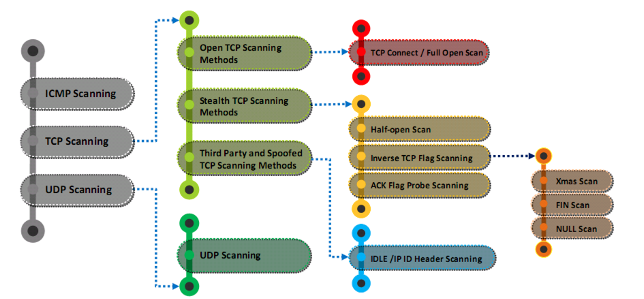
\includegraphics[width=0.78\textwidth,height=0.6\textheight,keepaspectratio]{img/sl026_1.png}
\end{center}
\end{frame}

\begin{frame}[allowframebreaks]{Escaneo de puertos}
\small
  \begin{itemize}
  \item IMPORTANTE: al realizar escaneos de sistemas en red a nivel TCP/IP, es completamente necesario analizar tanto los puertos TCP como UDP.
  \item Esquema de conexión TCP:
  \end{itemize}
\begin{center}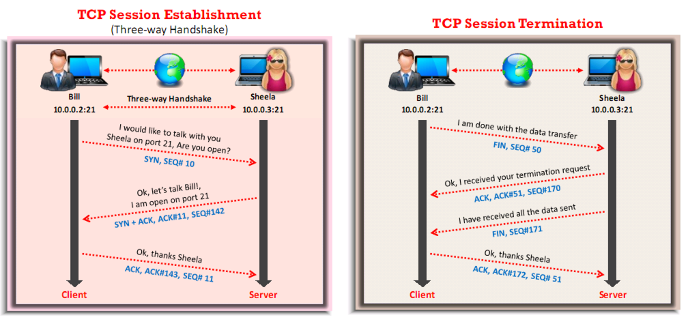
\includegraphics[width=0.78\textwidth,height=0.6\textheight,keepaspectratio]{img/sl023_1.png}
\end{center}
\end{frame}

\begin{frame}[allowframebreaks]{Escaneo de puertos}
  \small
  Flags del protocolo TCP:
\begin{center}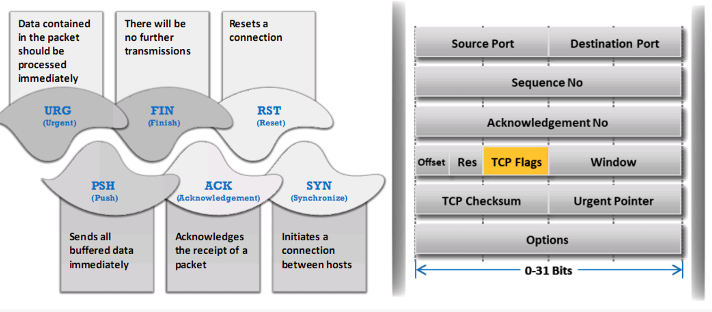
\includegraphics[width=0.78\textwidth,height=0.6\textheight,keepaspectratio]{img/sl024_1.png}
\end{center}
\end{frame}


\begin{frame}[allowframebreaks,fragile]{Escaneo de hosts y de puertos}
\small
  \begin{itemize}
  \item Lo primero que debemos hacer es detectar cuáles son los sistemas vivos en una determinada red. En caso de no encontrarnos en la misma red que los objetivos, podremos realizar los siguientes tipos de escaneo:
    \begin{itemize}
    \item ICMP Scan: utiliza paquetes ICMP para detectar si un equipo está vivo. En caso de existir medidas de seguridad o firewalls entre el auditor y el objetivo es posible que estos datos no sean verídicos.
      \begin{itemize}
      \item \verb|nmap -sn [IP]|
      \end{itemize}
    \item Ping Sweep: básicamente es un barrido de ICMP scan en un determinado rango de direcciones IP.
      \begin{itemize}
      \item \verb|nmap -sn [RANGO DE RED]| \quad (la opción \verb|-sP| es el nombre antiguo de \verb|-sn|)
      \end{itemize}
    \end{itemize}
  \end{itemize}
\end{frame}


\begin{frame}{Escaneo de puertos}
\small
  \begin{itemize}
  \item La herramienta Nmap cuenta con multitud de tipos de escaneos diferentes:
    \begin{itemize}
    \item TCP Scan (Connect Scan): realiza una conexión completa con cada puerto que comprueba. Es un escaneo lento y permite al sistema objetivo detectar más fácilmente el origen del escaneo.
    \item Inicialmente estos escaneos tenían una tasa de detección mayor; hoy en día es igual que la de otros escaneos como el SYN Scan.
    \end{itemize}
  \end{itemize}
\begin{center}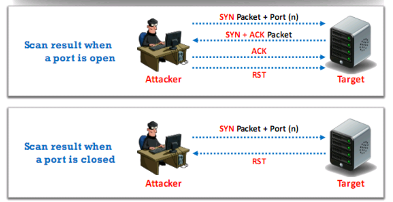
\includegraphics[width=0.7\textwidth,height=0.45\textheight,keepaspectratio]{img/sl029_1.png}
\end{center}
\end{frame}

\begin{frame}[allowframebreaks]{Escaneo de puertos}
\small
  \begin{itemize}
  \item SYN Scan (Half-scan): este tipo de escaneo es uno de los más rápidos y silenciosos. El auditor únicamente envía un paquete SYN y se queda a la espera de la respuesta. Una vez la recibe, no contesta con un ACK.
  \end{itemize}
\begin{center}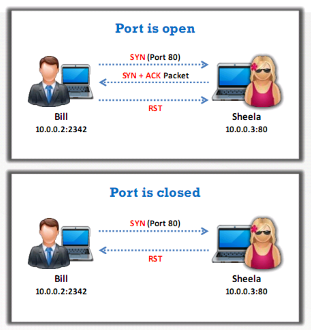
\includegraphics[width=0.78\textwidth,height=0.6\textheight,keepaspectratio]{img/sl030_1.png}
\end{center}
\end{frame}

\begin{frame}[allowframebreaks]{Escaneo de puertos}
\small
  \begin{itemize}
  \item ACK Scan: este escaneo es opuesto al anterior. En este caso el auditor únicamente envía un paquete ACK, lo cual sería erróneo según el protocolo. Si el servidor responde, es que el servicio está a la escucha.
  \item En caso de existir firewalls stateful, estos comprobarán que no se generen paquetes ACK sin existir antes paquetes SYN/ACK. Esto impide poder realizar este tipo de escaneos de forma correcta.
  \end{itemize}
\begin{center}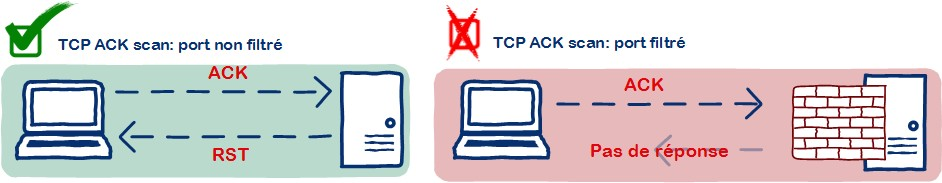
\includegraphics[width=0.78\textwidth,height=0.6\textheight,keepaspectratio]{img/sl031_1.jpg}
\end{center}
\end{frame}

\begin{frame}[allowframebreaks]{Escaneo de puertos}
\small
  \begin{itemize}
  \item UDP Scan: igual de importantes son los escaneos en los puertos UDP que en TCP, es por ello que en toda auditoría deben ser comprobados. En este caso, el funcionamiento suele ser bastante más lento que en TCP.
  \item Si el paquete se envía a un puerto cerrado, el sistema responderá con un mensaje ICMP de destino inalcanzable.
  \end{itemize}
\begin{center}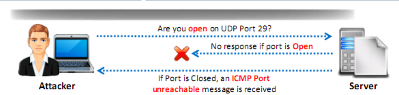
\includegraphics[width=0.78\textwidth,height=0.6\textheight,keepaspectratio]{img/sl032_1.png}
\end{center}
\end{frame}

\begin{frame}{Escaneo de puertos}
\small
  \begin{itemize}
  \item En caso de que existan medidas de seguridad, es posible utilizar otros escaneos alternativos, basados en la implementación de la pila TCP/IP. Los principales tipos son:
    \begin{itemize}
    \item NULL Scan: envía los paquetes a cada puerto escaneado sin ningún flag marcado.
    \item FIN Scan: envía los paquetes a cada puerto únicamente con el flag FIN marcado.
    \item XMAS Scan: envía los paquetes a cada puerto con todos los flags marcados.
    \item SSDP Scan: el protocolo SSDP (Simple Service Discovery Protocol) trabaja junto con el protocolo UPnP para detectar dispositivos plug and play.
    \end{itemize}
  \end{itemize}
\begin{center}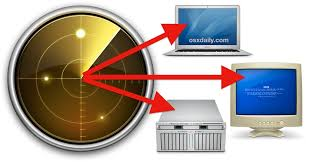
\includegraphics[width=0.5\textwidth,height=0.35\textheight,keepaspectratio]{img/sl035_1.jpg}
\end{center}
\end{frame}

\begin{frame}[allowframebreaks]{Ejercicio}
\small
\begin{center}
\includegraphics[width=0.78\textwidth,height=0.6\textheight,keepaspectratio]{img/sl036_1.jpg}
\end{center}
  \begin{itemize}
  \item Realiza diferentes tipos de escaneo de puertos con la herramienta Nmap frente a la distribución metasploitable2 y compara las salidas de cada uno de ellos. ¿Con qué tipo de escaneo obtienes mejores resultados?
  \end{itemize}
\end{frame}

\begin{frame}[allowframebreaks,fragile]{Fingerprinting}
\small
  \begin{itemize}
  \item Una vez el auditor ha detectado cuáles son los puertos abiertos, es el momento de comprobar el tipo de servicio y versión que está corriendo en ellos.
    \begin{itemize}
    \item Tipo de servicio: HTTP, FTP, SSH, Telnet, DNS, etcétera. A veces ocurre que el SSH no está en el puerto 22 o el HTTP no está en el puerto 80, por lo que es importante determinarlo.
    \item Versión: 1.0, 2.0, 3.0, etcétera.
    \end{itemize}
  \item Nmap permite realizar este tipo de fingerprinting de manera automática, y es capaz de detectar la versión de los servicios que hay corriendo en los puertos abiertos.
    \begin{itemize}
    \item Fingerprinting de servicios (\verb|-sV|).
    \item Scripts para fingerprinting (\verb|-sC|). Esto es realmente enumeración, y se verá más en profundidad en el tema 2.3.
    \end{itemize}
  \item Además del fingerprinting de servicios, es interesante también determinar el fingerprinting del sistema operativo y su versión.
    \begin{itemize}
    \item Fingerprinting de sistema operativo (\verb|-O|).
    \end{itemize}
  \end{itemize}
\end{frame}


\begin{frame}[allowframebreaks,fragile]{Nmap}
\small
  \begin{itemize}
  \item Existen otras muchas opciones útiles dentro de Nmap. A continuación se detallan algunas de ellas:
    \begin{itemize}
    \item Definir los puertos a escanear (\verb|-p|):
      \begin{itemize}
      \item Todos los puertos: \verb|-p-|
      \item Un rango: \verb|-p 1-65535|
      \item Una lista concreta: \verb|-p 80,443,8080,8443|
      \item Top principal de puertos: \verb|--top-ports [número]|
      \end{itemize}
    \item Modificar el puerto de origen de los escaneos (\verb|-g|): \verb|-g 80|
    \item Modo verbose: \verb|-v|
    \item Modo agresivo (\verb|-A|): equivale a \verb|-sV -O -sC --traceroute|
    \item Salida: \verb|-oG| (grep), \verb|-oN| (normal), \verb|-oX| (XML), \verb|-oA| (todos)
    \end{itemize}
  \end{itemize}
\end{frame}

\begin{frame}[allowframebreaks,fragile]{Nmap}
\small
Nmap: referencia rápida de comandos
  \begin{itemize}
  \item Descubrimiento de hosts:
    \begin{itemize}
    \item \verb|nmap -sn 192.168.1.0/24| --- ping sweep (sin escaneo de puertos)
    \item \verb|nmap -sn -PR 192.168.1.0/24| --- ARP scan en red local (más fiable)
    \end{itemize}
  \item Escaneo de puertos:
    \begin{itemize}
    \item \verb|nmap -sS IP| --- SYN scan, rápido y semisilencioso (requiere root)
    \item \verb|nmap -sT IP| --- TCP Connect, sin privilegios de root
    \item \verb|nmap -sU -p 53,161,500 IP| --- UDP scan en puertos clave
    \item \verb|nmap -p- IP| --- todos los puertos (1-65535)
    \item \verb|nmap --top-ports 1000 IP| --- los 1000 puertos más comunes
    \end{itemize}
  \item Fingerprinting y scripts:
    \begin{itemize}
    \item \verb|nmap -sV IP| --- versión de servicios
    \item \verb|nmap -O IP| --- sistema operativo (requiere root)
    \item \verb|nmap -A IP| --- agresivo: OS + versión + scripts + traceroute
    \item \verb|nmap -sC IP| --- scripts por defecto
    \item \verb|nmap --script vuln IP| --- buscar vulnerabilidades conocidas
    \end{itemize}
  \item Salida:
    \begin{itemize}
    \item \verb|nmap -oA nombre IP| --- exportar en \verb|.nmap|, \verb|.gnmap| y \verb|.xml| a la vez
    \item \verb@nmap -oG - IP | grep open@ --- salida grepable en tiempo real
    \end{itemize}
  \end{itemize}
\end{frame}

\begin{frame}[allowframebreaks]{Ejercicio}
\small
\begin{center}
\includegraphics[width=0.78\textwidth,height=0.6\textheight,keepaspectratio]{img/sl041_1.jpg}
\end{center}
  \begin{itemize}
  \item Identifica qué tipos de sistemas (fingerprinting OS) hay en tu red y, para cada puerto abierto, qué servicio y qué versión hay detrás de cada servicio activo (fingerprinting).
  \item También puedes hacerlo frente a la distribución metasploitable2.
  \end{itemize}

\end{frame}

\begin{frame}[allowframebreaks]{Fingerprinting mediante TTL}
\small
  \begin{itemize}
  \item Para determinar el sistema operativo de un equipo mediante el TTL (Time To Live), debes enviar un paquete ICMP con el comando ping.
  \item El valor de TTL recibido en la respuesta te permite identificar el sistema operativo base según el número de saltos que haya recorrido en la red.
  \item Valores iniciales de TTL por sistema operativo. Cada sistema operativo asigna un valor predeterminado de fábrica al salir el paquete:
    \begin{itemize}
    \item Linux / Unix / macOS: el TTL inicial suele ser 64.
    \item Windows: el TTL inicial suele ser 128.
    \item Dispositivos de red (Cisco / Solaris): el TTL inicial suele ser 255.
    \end{itemize}
  \end{itemize}
\end{frame}

\begin{frame}{Ejercicio}
\small
\begin{center}
\includegraphics[width=0.6\textwidth,height=0.45\textheight,keepaspectratio]{img/sl042_1.jpg}
\end{center}
  \begin{itemize}
  \item Determina el sistema operativo de una máquina observando el valor TTL con el que responde a un ping.
  \item Realiza un script en Python para determinar el sistema operativo de una máquina a partir del TTL de respuesta de los paquetes.
  \end{itemize}
\end{frame}


\begin{frame}{Fingerprinting mediante banner grabbing}
\small
  \begin{itemize}
  \item Utilizar comunicaciones ``en crudo'' frente a los servicios, usando protocolos (FTP, Telnet, etc.) o herramientas (netcat, etc.), para obtener la versión que hay corriendo en dichos servicios.
  \item Ejemplos:
    \begin{itemize}
    \item ftp
    \item telnet
    \item \href{https://github.com/jaygreig86/dmitry}{Dmitry}
    \end{itemize}
  \end{itemize}
\begin{center}
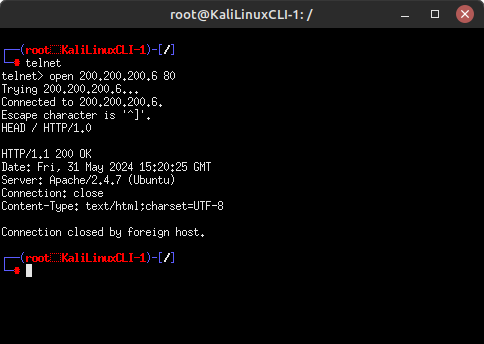
\includegraphics[width=0.42\textwidth,height=0.34\textheight,keepaspectratio]{img/banner-grabbing-http.png}\\
{\tiny Ejemplo: banner grabbing de un servidor HTTP con telnet. Fuente: \href{https://eaglepubs.erau.edu/}{Embry-Riddle Aeronautical University}}
\end{center}
\end{frame}

\section{Netcat}

\begin{frame}[allowframebreaks,fragile]{Netcat}
\small
  \begin{itemize}
  \item Netcat es un servicio\slash aplicación para la comunicación basado en una filosofía cliente\slash servidor.
  \item Netcat (conocido por su comando \verb|nc|) es una herramienta de línea de comandos que sirve para leer y escribir datos a través de conexiones de red utilizando los protocolos TCP o UDP.
    \begin{itemize}
    \item Servidor: se crea un proceso en escucha en un puerto.
      \begin{itemize}
      \item \verb|nc -lvp <puerto>|
      \end{itemize}
    \item Cliente: se usa netcat para comunicarse, en claro, con el servidor que está a la escucha:
      \begin{itemize}
      \item \verb|nc <ip> <puerto>|
      \end{itemize}
    \end{itemize}
  \item Documentación: \href{https://www.hackingtutorials.org/networking/hacking-with-netcat-part-1-the-basics/}{parte 1}, \href{https://www.hackingtutorials.org/networking/hacking-netcat-part-2-bind-reverse-shells/}{parte 2}, \href{https://www.hackingtutorials.org/networking/hacking-with-netcat-part-3-advanced-techniques/}{parte 3}
  \item netcat en PowerShell:
    \begin{itemize}
    \item \href{https://github.com/besimorhino/powercat}{powercat}
    \end{itemize}
  \end{itemize}
\end{frame}

\begin{frame}[allowframebreaks]{Netcat}
\small
  Netcat para banner grabbing y para la transferencia de archivos:
\begin{center}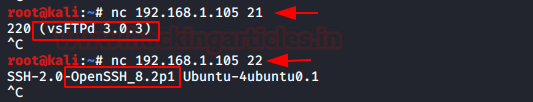
\includegraphics[width=0.62\textwidth,height=0.42\textheight,keepaspectratio]{img/sl046_1.png}
\end{center}
\begin{center}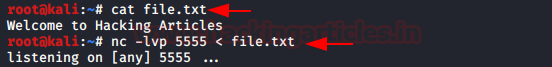
\includegraphics[width=0.62\textwidth,height=0.42\textheight,keepaspectratio]{img/sl046_2.png}
\end{center}
\begin{center}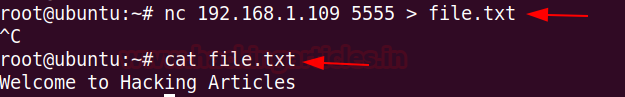
\includegraphics[width=0.62\textwidth,height=0.42\textheight,keepaspectratio]{img/sl046_3.png}
\end{center}
\end{frame}


\begin{frame}[allowframebreaks]{Netcat}
\small
Netcat para ejecución de shells:
\begin{center}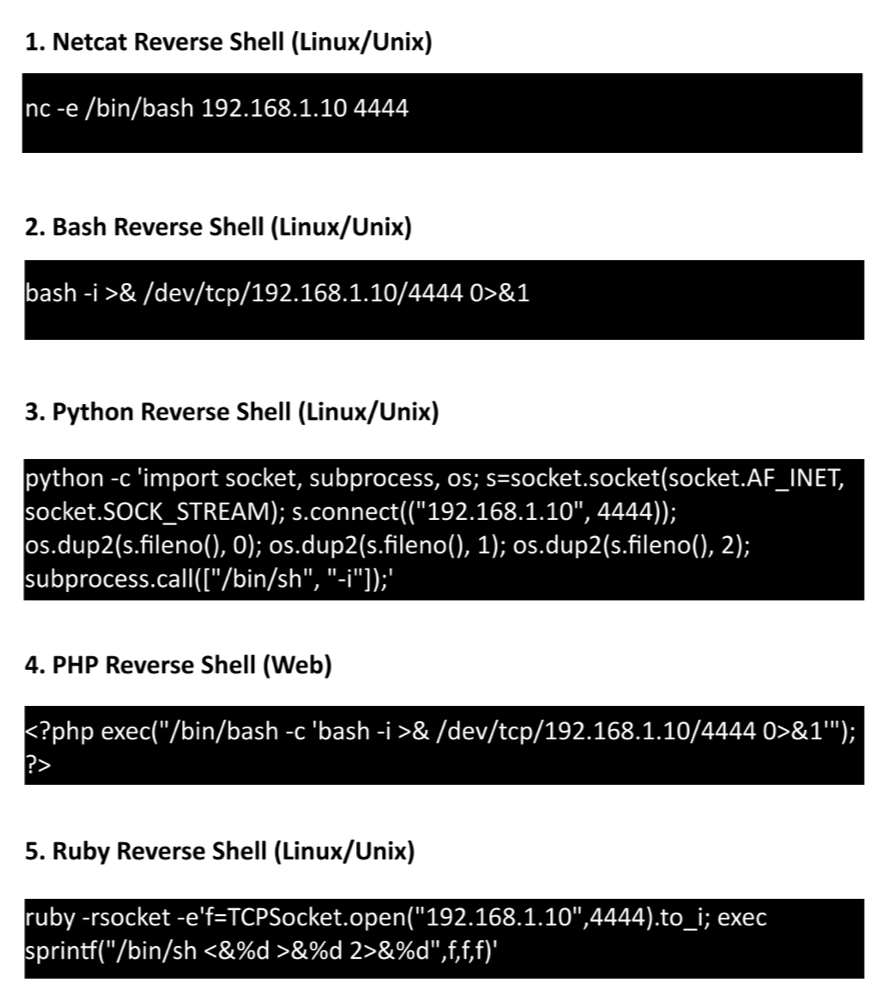
\includegraphics[width=0.78\textwidth,height=0.6\textheight,keepaspectratio]{img/sl047_1.png}
\end{center}
\end{frame}

\begin{frame}[allowframebreaks,fragile]{Netcat}
\small
  \begin{itemize}
  \item Una de las funciones más interesantes de Netcat es la capacidad de transferir directorios completos, comprimidos al vuelo, entre máquinas.
  \item En la máquina que envía:
    \begin{itemize}
    \item \verb@tar -czf - /ruta/directorio | nc 192.168.1.50 4444@
    \item Este comando comprime el directorio indicado y lo transmite por el puerto 4444.
    \end{itemize}
  \item En la máquina que recibe:
    \begin{itemize}
    \item \verb@nc -l -p 4444 | tar -xzf -@
    \item Este comando recibe el flujo comprimido y lo extrae en el directorio actual del equipo destino.
    \end{itemize}
  \end{itemize}
\end{frame}


\begin{frame}[fragile]{Netcat}
\small
Netcat también nos puede servir para escanear puertos:
  \begin{itemize}
  \item Opciones:
    \begin{itemize}
    \item \verb|-z| se utiliza para escanear.
    \item \verb|-v| para añadir verbosidad.
    \item \verb|-w 1| se utiliza para establecer el tiempo de espera de cada conexión en 1 segundo.
    \item \verb|1-10000| define qué puertos escanear.
    \end{itemize}
  \end{itemize}
\begin{center}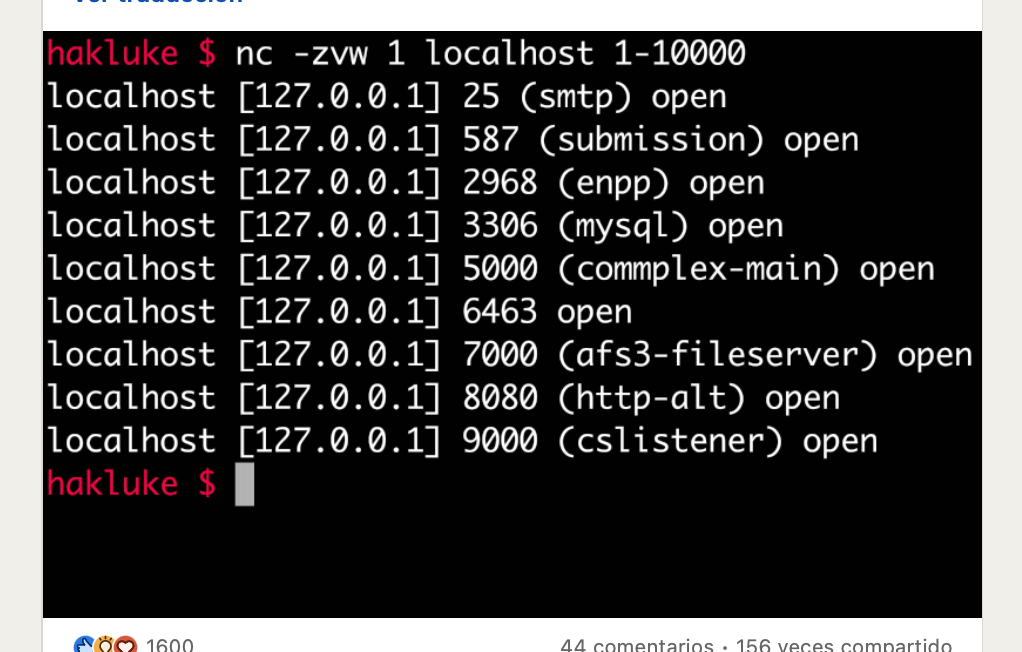
\includegraphics[width=0.55\textwidth,height=0.34\textheight,keepaspectratio]{img/sl051_1.png}
\end{center}
\end{frame}

\begin{frame}[allowframebreaks]{Ejercicio: TryHackMe}
\small
\begin{center}
\includegraphics[width=0.78\textwidth,height=0.6\textheight,keepaspectratio]{img/sl052_1.jpg}
\end{center}
  \begin{itemize}
  \item Resuelve esta \href{https://tryhackme.com/room/nmap01}{room} sobre Nmap y netcat en TryHackMe.
  \end{itemize}
\end{frame}

\begin{frame}[allowframebreaks]{Ejercicio}
\small
\begin{center}
\includegraphics[width=0.78\textwidth,height=0.6\textheight,keepaspectratio]{img/sl053_1.jpg}
\end{center}
  \begin{itemize}
  \item Haz varias pruebas con la herramienta netcat entre la máquina Kali y la máquina metasploitable2.
  \end{itemize}
\end{frame}


\section{Nmap Scripting Engine}

\begin{frame}[allowframebreaks]{Nmap Scripting Engine}
\small
  \begin{itemize}
  \item La herramienta Nmap dispone de unas extensiones, denominadas NSE (Nmap Scripting Engine), que son de código abierto: cualquiera puede aportar su script a la comunidad. Son útiles para realizar labores más avanzadas que las de escaneo y fingerprinting propias de Nmap.
  \item Con los NSE se pueden hacer acciones de:
    \begin{itemize}
    \item OSINT / footprinting
    \item Análisis de vulnerabilidades
    \item Fuzzing / enumeración
    \item Interacción con servicios
    \item Ataques de fuerza bruta
    \end{itemize}
  \item Documentación: \href{https://nmap.org/nsedoc/}{nsedoc}
  \end{itemize}
\end{frame}

\begin{frame}[allowframebreaks]{Nmap Scripting Engine}
\small
  \begin{itemize}
  \item Repositorios en GitHub:
    \begin{itemize}
    \item \href{https://github.com/emadshanab/Nmap-NSE-scripts-collection}{Nmap-NSE-scripts-collection}
    \end{itemize}
  \item Los scripts se categorizan en las siguientes clases:
  \end{itemize}
\begin{center}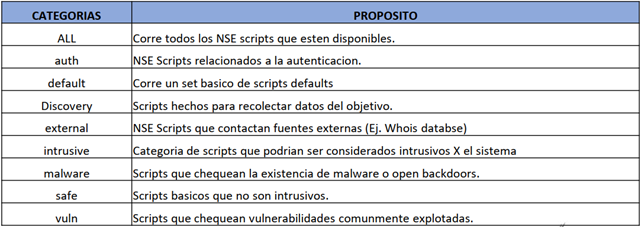
\includegraphics[width=0.78\textwidth,height=0.6\textheight,keepaspectratio]{img/sl056_1.png}
\end{center}
\end{frame}

\begin{frame}[allowframebreaks,fragile]{Nmap Scripting Engine}
\small
  \begin{itemize}
  \item En Kali los puedes encontrar con:
    \begin{itemize}
    \item \verb|locate *.nse|
    \end{itemize}
  \item Ejecutar scripts individuales:
    \begin{itemize}
    \item \verb|nmap --script [script.nse] [target]|
    \end{itemize}
  \item Ejecutar scripts por categorías:
    \begin{itemize}
    \item \verb|nmap --script [categoria] [target]|
    \end{itemize}
  \item Ejecutar scripts de múltiples categorías:
    \begin{itemize}
    \item \verb|nmap --script [categoria1,categoria2,...] [target]|
    \end{itemize}
  \item Solucionar problemas de scripts:
    \begin{itemize}
    \item \verb|nmap --script [script] --script-trace [target]|
    \end{itemize}
  \item Actualizar la base de datos de scripts:
    \begin{itemize}
    \item \verb|nmap --script-updatedb|
    \end{itemize}
  \end{itemize}
\end{frame}

\begin{frame}[allowframebreaks]{Nmap Scripting Engine}
\small
  \begin{itemize}
  \item Encontrar vhosts alojados en la misma IP. Ejemplos: \href{https://pentestlab.blog/2013/02/16/information-gathering-with-nmap/}{lectura 1}, \href{https://hackertarget.com/7-nmap-nse-scripts-recon/}{lectura 2}, \href{https://www.welivesecurity.com/la-es/2015/02/12/auditando-nmap-scripts-escanear-vulnerabilidades/}{lectura 3}.
  \end{itemize}
\begin{center}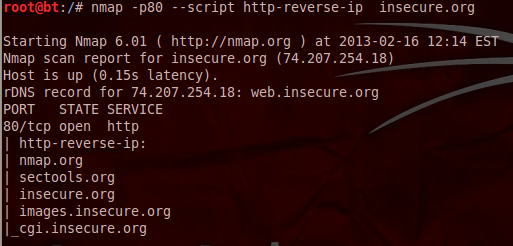
\includegraphics[width=0.78\textwidth,height=0.6\textheight,keepaspectratio]{img/sl058_1.png}
\end{center}
\end{frame}

\begin{frame}[allowframebreaks]{Nmap Scripting Engine}
\small
  \begin{itemize}
  \item Detectar la vulnerabilidad EternalBlue (MS17-010), que fue la que explotaba el malware WannaCry.
  \end{itemize}
\begin{center}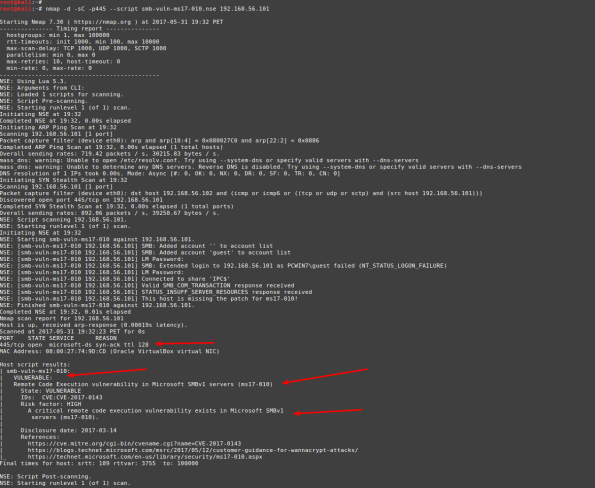
\includegraphics[width=0.78\textwidth,height=0.6\textheight,keepaspectratio]{img/sl059_1.png}
\end{center}
\end{frame}

\begin{frame}[allowframebreaks]{Nmap Scripting Engine}
\small
  \begin{itemize}
  \item Fingerprinting de servicios y versiones de software con NSE:
  \end{itemize}
\begin{center}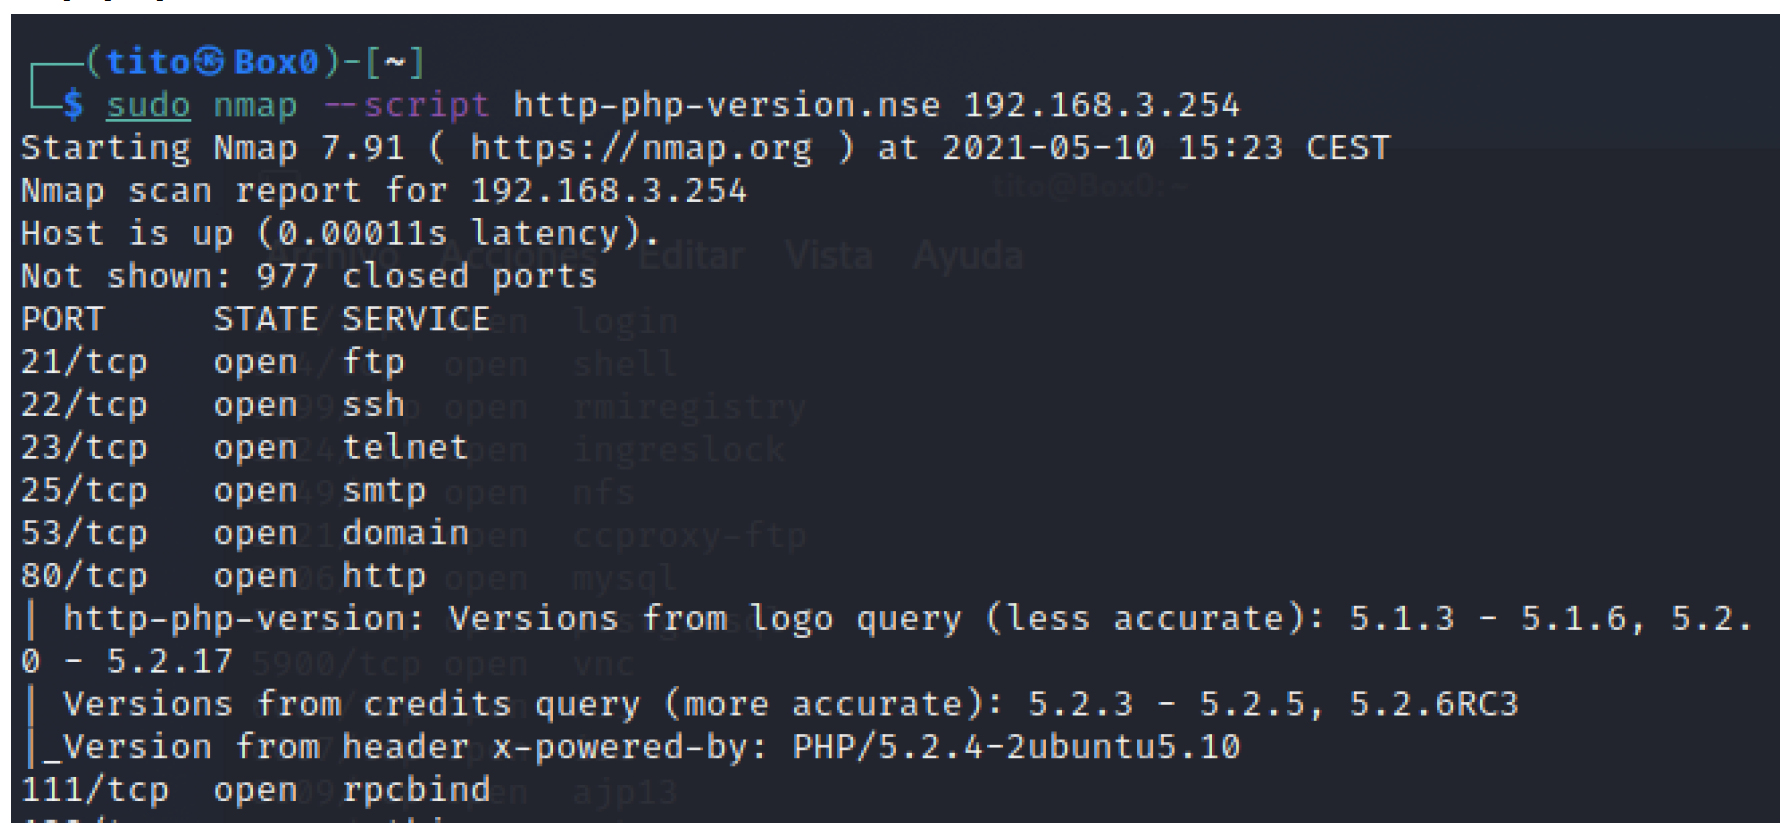
\includegraphics[width=0.78\textwidth,height=0.6\textheight,keepaspectratio]{img/sl060_1.png}
\end{center}
\end{frame}

\begin{frame}[allowframebreaks]{Nmap Scripting Engine}
\small
Herramientas:
  \begin{itemize}
  \item \href{https://www.kitploit.com/2018/04/autonse-massive-nse-nmap-scripting.html}{autoNSE}
  \end{itemize}
\end{frame}


\begin{frame}{Ejercicio}
\small
\begin{center}
\includegraphics[width=0.6\textwidth,height=0.45\textheight,keepaspectratio]{img/sl061_1.jpg}
\end{center}
  \begin{itemize}
  \item Lanza al menos un script NSE de cada una de las categorías NSE frente a un objetivo a tu elección (o la máquina metasploitable2).
  \item Nota: puede ser de tu red interna o una IP externa.
  \end{itemize}
\end{frame}

\section{Técnicas de Evasión}

\begin{frame}[allowframebreaks]{Técnicas de Evasión}
\small
  \begin{itemize}
  \item La mejor contramedida frente a los escaneos es introducir un firewall o un sistema de detección de intrusiones (IDS) que disponga de firmas para la detección de los reconocimientos.
  \item Frente a la protección que ofrecen los firewalls y los IDS, existen diferentes técnicas que intentan saltarse dicha protección, por ejemplo, los distintos tipos de escaneo:
    \begin{itemize}
    \item Fragmentación de paquetes
    \item Modificación de rutas
    \item Modificación de direcciones IP o MAC
    \item Proxies
    \item Resumen de técnicas: \href{https://www.elladodelmal.com/2019/10/tecnicas-de-escaneo-y-evasion-con-namp.html}{El lado del mal}
    \end{itemize}
  \end{itemize}
\end{frame}

\begin{frame}[allowframebreaks,fragile]{Técnicas de Evasión}
\small
Distintos tipos de escaneo:
  \begin{itemize}
  \item Como se ha visto a lo largo de esta sección, los diferentes tipos de escaneos pueden permitir la evasión de un firewall.
  \item Por ejemplo, un firewall puede filtrar paquetes que no pertenezcan a una conexión previamente establecida, pero con el escaneo XMAS, que tiene ciertos flags del paquete TCP activos, se podría evadir esa regla de filtrado.
  \item Señales atípicas (\verb|-sN|, \verb|-sF|, \verb|-sX|): envía paquetes con combinaciones raras de flags (NULL, FIN o XMAS) para atravesar ciertos firewalls sin levantar alertas básicas.
  \end{itemize}
\end{frame}

\begin{frame}[fragile]{Técnicas de Evasión}
\small
Fragmentación de paquetes y señuelos:
  \begin{itemize}
  \item La idea reside en trocear la cabecera del paquete a partir del campo MTU que introduce la pila TCP/IP. Por tanto, un escaneo que se podría hacer con unos pocos paquetes se realiza usando muchos más de tamaño más pequeño. Esto hace que el firewall intermedio no sea capaz de interpretar la cabecera completa, puesto que el paquete se reconstruye en el destino y no en el firewall.
    \begin{itemize}
    \item Fragmentación en Nmap: \verb|-f| o \verb|--mtu|
    \end{itemize}
  \end{itemize}
\begin{center}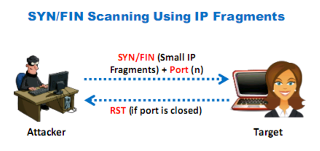
\includegraphics[width=0.5\textwidth,height=0.32\textheight,keepaspectratio]{img/sl065_1.png}
\end{center}
\end{frame}

\begin{frame}[allowframebreaks,fragile]{Técnicas de Evasión}
\small
  \begin{itemize}
  \item La fragmentación divide paquetes para que el IDS/firewall no pueda inspeccionarlos.
  \item Ejemplos de comandos Nmap para fragmentación y MTU:
    \begin{itemize}
    \item \verb|nmap -f IP| --- fragmentos de 8 bytes (escapa del DPI básico)
    \item \verb|nmap -ff IP| --- fragmentos de 16 bytes
    \item \verb|nmap --mtu 8 IP| --- MTU personalizado (debe ser múltiplo de 8)
    \end{itemize}
  \item Combinado con otros tipos de escaneo:
    \begin{itemize}
    \item \verb|nmap -sS -f --mtu 8 -p 80,443,8080 192.168.1.1|
    \item \verb|nmap -sS -ff -T2 -p- 192.168.1.1|
    \end{itemize}
  \item Por qué funciona y cuáles son sus límites:
    \begin{itemize}
    \item El firewall recibe fragmentos aislados $\rightarrow$ no puede reconstruir la cabecera TCP completa.
    \item El host destino sí reconstruye el paquete $\rightarrow$ la conexión funciona correctamente.
    \item Los IDS modernos con \emph{packet reassembly} no son engañados por esta técnica por sí sola.
    \item Conviene combinarla siempre con \verb|--data-length| o \verb|-D| para mayor efectividad.
    \end{itemize}
  \end{itemize}
\end{frame}

\begin{frame}[allowframebreaks]{Técnicas de Evasión}
\small
Modificación de rutas:
  \begin{itemize}
  \item Los paquetes siguen sus rutas para llegar al destino a partir del origen.
  \item Esta técnica reside en especificar la ruta que debe seguir el paquete para evadir el firewall / IDS.
  \end{itemize}
\begin{center}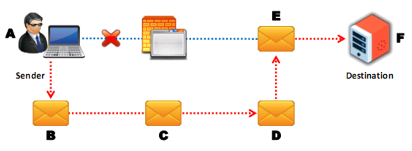
\includegraphics[width=0.78\textwidth,height=0.6\textheight,keepaspectratio]{img/sl067_1.png}
\end{center}
\end{frame}

\begin{frame}[allowframebreaks,fragile]{Técnicas de Evasión}
\small
  \begin{itemize}
  \item Modificación de direcciones IP o MAC:
    \begin{itemize}
    \item Consiste en cambiar la IP origen del paquete para evadir el firewall / IDS. De esta manera, los sistemas que filtran una IP no son capaces de determinar si el paquete ha salido de la IP bloqueada o no.
    \item También se puede aplicar a la dirección física MAC.
      \begin{itemize}
      \item IP y MAC falsas en Nmap: \verb|-S| y \verb|--spoof-mac|
      \end{itemize}
    \end{itemize}
  \end{itemize}
\begin{center}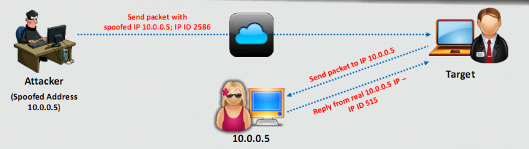
\includegraphics[width=0.78\textwidth,height=0.6\textheight,keepaspectratio]{img/sl068_1.png}
\end{center}
\end{frame}

\begin{frame}[allowframebreaks,fragile]{Técnicas de Evasión}
\small
Decoy Scan y Zombie Scan: anonimización del origen
  \begin{itemize}
  \item Decoy Scan (\verb|-D|): envía el escaneo mezclado con direcciones IP falsas para ocultar el origen real del atacante.
  \item El IDS/firewall ve múltiples orígenes y no puede determinar cuál es el atacante real.
  \item Ejemplos:
    \begin{itemize}
    \item \verb|nmap -D RND:10 IP| --- 10 IPs aleatorias como señuelo
    \item \verb|nmap -D IP1,IP2,ME,IP3 IP| --- \verb|ME| = posición de tu IP real entre los señuelos
    \item \verb|nmap -D RND:5 -sS -f IP| --- combinado con SYN scan y fragmentación
    \end{itemize}
  \item Zombie (Idle) Scan (\verb|-sI|): anonimato total. La IP real nunca aparece en el tráfico hacia el objetivo.
  \item Ejemplo:
    \begin{itemize}
    \item \verb|nmap -sI zombie_IP:puerto IP_objetivo|
    \end{itemize}
  \end{itemize}
\end{frame}


\begin{frame}[allowframebreaks]{Técnicas de Evasión}
  \small
  Cómo funciona el Zombie Scan (paso a paso):
  \begin{enumerate}
  \item Nmap consulta el IPID actual del zombie (predictor de secuencia).
  \item Nmap envía un SYN al objetivo falsificando la IP del zombie como origen.
  \item Puerto abierto $\rightarrow$ el objetivo envía SYN/ACK al zombie $\rightarrow$ el zombie responde RST (IPID +2).
  \item Puerto cerrado $\rightarrow$ el objetivo envía RST al zombie $\rightarrow$ el zombie lo descarta (IPID +1).
  \item Nmap vuelve a consultar el IPID del zombie y deduce si el puerto estaba abierto.
  \end{enumerate}
\end{frame}


\begin{frame}[allowframebreaks,fragile]{Técnicas de Evasión}
\small
Proxies
  \begin{itemize}
  \item Un proxy es un servicio que hace de intermediario en la comunicación entre dos hosts, de tal manera que el destino o los dispositivos de detección identifican que la petición la hace el proxy (la IP del proxy), y este esconde al emisor real de la petición.
  \item Anonimización completa vía Proxychains + TOR. Ejemplo:
    \begin{itemize}
    \item \verb|proxychains nmap -sT -Pn IP| --- solo TCP Connect funciona por TOR
    \end{itemize}
  \end{itemize}
\begin{center}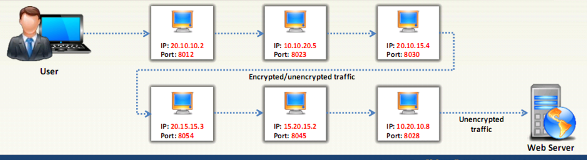
\includegraphics[width=0.78\textwidth,height=0.6\textheight,keepaspectratio]{img/sl070_1.png}
\end{center}
\end{frame}

\begin{frame}[allowframebreaks,fragile]{Técnicas de Evasión}
\small
Puerto de origen y timing:
  \begin{itemize}
  \item Puerto de origen: simular tráfico legítimo (\verb|-g| / \verb|--source-port|).
  \item Muchos firewalls permiten tráfico proveniente de puertos de servicios conocidos. Esto se puede simular con Nmap, por ejemplo:
    \begin{itemize}
    \item \verb|nmap -g 53 IP| --- simula consulta DNS saliente (puerto 53)
    \item \verb|nmap --source-port 80 IP| --- simula tráfico web HTTP
    \item \verb|nmap -g 443 -sS IP| --- simula HTTPS, muy eficaz contra firewalls permisivos
    \end{itemize}
  \item Timing: evitar la detección por volumen o frecuencia. Ejemplos:
    \begin{itemize}
    \item \verb|nmap -T0 IP| --- paranoid: 1 sonda cada 5 min (máximo sigilo)
    \item \verb|nmap -T1 IP| --- sneaky: 1 sonda cada 15 s
    \item \verb|nmap --scan-delay 2s IP| --- demora manual entre sondas
    \item \verb|nmap --max-rate 10 IP| --- máximo 10 paquetes/segundo
    \end{itemize}
  \end{itemize}
\end{frame}

\begin{frame}[allowframebreaks,fragile]{Técnicas de Evasión}
\small
Datos adicionales
  \begin{itemize}
  \item Confundir la inspección profunda (DPI). Ejemplos:
    \begin{itemize}
    \item \verb|nmap --data-length 25 IP| --- añade 25 bytes aleatorios al paquete
    \item \verb|nmap --data-length 100 -sS IP| --- hace que los paquetes parezcan tráfico real
    \end{itemize}
  \end{itemize}
\end{frame}

\begin{frame}[allowframebreaks]{Técnicas de Evasión}
\small
  \begin{itemize}
  \item Resumen de cómo lanzar estas opciones desde la herramienta Nmap:
    \begin{itemize}
    \item \href{https://youtu.be/-DEo9Ffq7UU}{Vídeo de documentación}
    \end{itemize}
  \end{itemize}
\begin{center}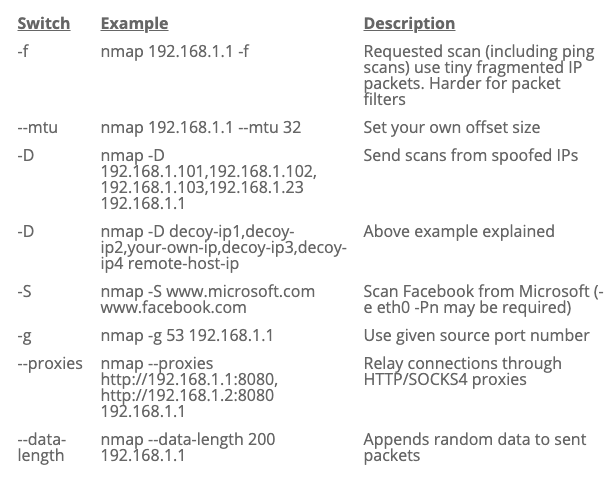
\includegraphics[width=0.78\textwidth,height=0.6\textheight,keepaspectratio]{img/sl072_1.png}
\end{center}
\end{frame}

\begin{frame}[allowframebreaks,fragile]{Técnicas de Evasión}
\small
Tabla resumen de técnicas Nmap:
  \begin{itemize}
  \item Fragmentación \verb|-f| / \verb|--mtu 8| $\rightarrow$ evade: DPI e inspección de paquetes
  \item Decoy \verb|-D RND:10| $\rightarrow$ evade: identificación del origen
  \item Zombie Scan \verb|-sI zombie_IP| $\rightarrow$ evade: todo (IP real invisible)
  \item Puerto origen \verb|-g 53| / \verb|--source-port| $\rightarrow$ evade: reglas por puerto fuente
  \item Timing \verb|-T0| / \verb|--scan-delay| $\rightarrow$ evade: detección por volumen/velocidad
  \item Datos adicionales \verb|--data-length 25| $\rightarrow$ evade: firmas de paquetes en IDS
  \item MAC spoofing \verb|--spoof-mac 0| $\rightarrow$ evade: filtros por dirección física
  \end{itemize}
\medskip
Comando combinado ``de bajo perfil'':
  \begin{itemize}
  \item {\scriptsize\verb|nmap -sS -f --mtu 8 -T1 -D RND:5 --source-port 443 --data-length 20 -Pn -oA scan IP|}
  \end{itemize}
Anonimización completa vía Proxychains + TOR:
  \begin{itemize}
  \item \verb|proxychains nmap -sT -Pn IP| --- solo TCP Connect funciona por TOR
  \end{itemize}
\end{frame}

\begin{frame}[allowframebreaks,fragile]{Detección de WAFs}
\small
  \begin{itemize}
  \item Usando los NSE de Nmap. Ejemplos:
    \begin{itemize}
    \item \verb|nmap --script http-waf-detect IP|
    \item \verb|nmap --script http-waf-fingerprint IP|
    \end{itemize}
  \item Cambio de User-Agent: por defecto, Nmap se identifica a sí mismo. Modifica esto usando \verb|--script-args http.useragent="Mozilla/5.0..."| para simular tráfico de un navegador legítimo.
  \item Inspección de cabeceras HTTP (análisis pasivo):
    \begin{itemize}
    \item Cabecera \verb|Server|: muchos WAF modifican esta cabecera revelando su identidad (por ejemplo, \verb|Server: cloudflare| o \verb|Server: BarracudaWAF|).
    \item Cabeceras personalizadas: algunos cortafuegos inyectan cabeceras propias en las respuestas HTTP, como \verb|X-Sucuri-ID|, \verb|X-CDN| o \verb|X-Protected-By|.
    \end{itemize}
  \end{itemize}
\end{frame}

\begin{frame}[allowframebreaks]{Detección de WAFs}
\small
  \begin{itemize}
  \item Herramientas:
    \begin{itemize}
    \item \href{https://github.com/EnableSecurity/wafw00f}{WafW00f}: envía solicitudes HTTP normales y alteradas para analizar las respuestas del servidor y las cookies, identificando casi cualquier WAF comercial o de código abierto.
    \item \href{https://github.com/Ekultek/WhatWaf}{WhatWaf}: modifica los payloads de los ataques para detectar qué tipo de reglas del WAF están bloqueando la solicitud y sugiere métodos de evasión (bypasses).
    \item \href{https://github.com/Y000o/Nmap/blob/main/Nmap_medio_Avanzado.md}{Nmap avanzado}
    \end{itemize}
  \end{itemize}
\end{frame}


\begin{frame}[allowframebreaks,fragile]{Ejercicio}
\small
\begin{center}
\includegraphics[width=0.78\textwidth,height=0.6\textheight,keepaspectratio]{img/sl074_1.jpg}
\end{center}
  \begin{itemize}
  \item Levanta dos máquinas Unix (Kali y metasploitable2, por ejemplo) y juega con los filtros iptables y las opciones de evasión de Nmap.
  \end{itemize}

\scriptsize
  \begin{itemize}
  \item \verb|sudo iptables -I INPUT -p tcp --tcp-flags ALL SYN -j REJECT --reject-with tcp-reset|
    \begin{itemize}
    \item Soluciones: \verb|nmap -sF|, \verb|nmap -sN|, \verb|nmap -sX|
    \item Limpiar las reglas: \verb|sudo iptables -F INPUT|
    \end{itemize}

  \item \verb|sudo iptables -I INPUT -p tcp -m length --length 40 -j REJECT --reject-with tcp-reset|
    \begin{itemize}
    \item \verb|sudo nmap -sF|
    \item \verb|-sS| funciona: son 44 bytes (\verb|--length 44|)
    \item \verb|sudo nmap --data-length 10|
    \end{itemize}

  \item Fragmentación de paquetes: \verb|-f|
  \item \verb|sudo iptables -I INPUT -p tcp -m length --length :256 -j REJECT --reject-with tcp-reset|
    \begin{itemize}
    \item \verb|nmap --data-length 300 <tu_objetivo>|
    \end{itemize}

  \item \verb|sudo iptables -I INPUT -p tcp -m ttl --ttl-lt 64 -j REJECT --reject-with tcp-reset|
    \begin{itemize}
    \item \verb|sudo nmap --ttl 65|
    \end{itemize}

  \item \verb|sudo iptables -I INPUT -p tcp -j REJECT --reject-with tcp-reset| (rechaza todo el tráfico TCP)
  \item \verb|sudo iptables -I INPUT -p tcp -j REJECT|
  \item \verb|sudo iptables -I INPUT -p tcp --sport 1337 -j ACCEPT|
    \begin{itemize}
    \item \verb|sudo nmap -g 1337|
    \end{itemize}

  \item Decoy: \verb|sudo iptables -I INPUT -p tcp -j LOG --log-prefix "atacker log" --log-level=4|
    \begin{itemize}
    \item \verb|nmap -sS -D ip,ME,ip -p 80 ipobjetivo|
    \item \verb|tail -f /var/log/syslog -n 40|
    \end{itemize}

  \item Filtrar por MAC: \verb|sudo iptables -A INPUT -m mac --mac-source 00:0F:EA:91:04:08 -j REJECT|
    \begin{itemize}
    \item \verb|sudo macchanger -r eth1|
    \item \verb|macchanger -s|
    \item O también: \verb|sudo nmap --spoof-mac Apple| (o poner la MAC concreta; \verb|0| $\rightarrow$ aleatoria)
    \end{itemize}
  \end{itemize}
\end{frame}

\begin{frame}[allowframebreaks]{Ejercicio}
\small
\begin{center}
\includegraphics[width=0.78\textwidth,height=0.6\textheight,keepaspectratio]{img/sl075_1.jpg}
\end{center}
  \begin{itemize}
  \item Resuelve la room \href{https://tryhackme.com/room/furthernmap}{furthernmap}.
  \end{itemize}
\end{frame}

\begin{frame}[plain]
  \begin{center}
    {\Huge\bfseries\color{uznavy} ¡Gracias!}\\[1em]
    {\large Seguridad en Sistemas Informáticos --- Tema 2.2}
  \end{center}
\end{frame}

\end{document}
